% ICML 2022 format. To compile on Overleaf:
%   1. Start a new project from the ICML 2022 template
%      (https://www.overleaf.com/latex/templates/icml2022-template/)
%   2. Replace the example.tex with this file.
%   3. Compile with pdflatex.

\documentclass{article}

\usepackage{microtype}
\usepackage{graphicx}
\usepackage{subfigure}
\usepackage{booktabs}
\usepackage{hyperref}

\usepackage[accepted]{icml2022}

\icmltitlerunning{Bias-Aware Resume-Job Matching}

\begin{document}

\twocolumn[
\icmltitle{Bias-Aware Resume-Job Matching: Auditing and Mitigating\\
Demographic Bias in Automated Hiring Systems}

\begin{icmlauthorlist}
\icmlauthor{Moksh Jain}{umbc}
\icmlauthor{Sai Satwika Reddy Kandula}{umbc}
\end{icmlauthorlist}

\icmlaffiliation{umbc}{Department of Computer Science, University of Maryland, Baltimore County}

\icmlcorrespondingauthor{Moksh Jain}{}
\icmlcorrespondingauthor{Sai Satwika Reddy Kandula}{}

\icmlkeywords{fairness, NLP, sentence embeddings, resume screening, counterfactual analysis}

\vskip 0.3in
]

\printAffiliationsAndNotice{}

\begin{abstract}
Automated resume-screening tools are used to rank candidates before a person looks at them. If those tools react to demographic cues that have nothing to do with the job, then people who are equally qualified may end up with different scores. In this project we build a small resume-job matcher with Sentence-BERT and check it with counterfactual resumes. Each counterfactual changes only one demographic signal at a time: the applicant's name, their pronouns, or their university. We measure how much the score moves. We also try blind screening as a mitigation, add a TF-IDF baseline, a compound-signal version where all three signals change at once, and a comparison with the FLAN-T5-base language model. We run paired Wilcoxon tests and bootstrap confidence intervals so the small differences are not over-claimed. Name changes produce the largest average score shift, followed by university and then pronouns. The blind-screening result is a useful upper bound but, as we explain, is forced toward zero by construction on our dataset. The LLM comparison shows that small instruction-tuned models can also flip their match label when only a demographic signal changes.
\end{abstract}

\section{Introduction}

Online job sites get a lot more applications than any company can read. To deal with this, hiring tools rank or filter resumes automatically before a person sees them. These tools help with volume, but they can also pick up patterns from past data that are not really about the job. If the score the tool gives changes when only the applicant's name or pronouns change, that is a sign the tool is sensitive to something it should not be.

This project looks at one of those tools: a Sentence-BERT based resume-job matcher. We use cosine similarity between resume and job embeddings as the matching score. We then change one demographic field in the resume at a time and measure how much the score moves. We compare to a TF-IDF baseline, try blind screening as a mitigation, and check what a small open-source language model (FLAN-T5-base) does on the same pairs.

\section{Problem and Motivation}

When you apply to a job online, a program almost always reads your resume first. Past research has shown that hiring is influenced by demographic cues even when qualifications are the same. \citet{bertrand2004emily} sent identical resumes with different first names and showed that resumes with white-sounding names got 50\% more callbacks. More recent work shows the same kind of effect in language-model-based screening~\cite{wilson2024gender}.

Our motivation is to build a small, working pipeline that you can actually run, and to use it to check whether the matching score reacts to demographic cues. Talking about bias in general is fine, but you learn more when you have a system in front of you and you can poke at it. We also try a basic mitigation step and ask whether it actually changes anything.

\section{Research Questions}

In our proposal we listed four questions. We were able to answer the first two well, made a partial answer for the third, and added a new one for the LLM that the instructor asked about. The original questions and the changes are listed in Section~\ref{sec:scope}.

\begin{enumerate}
    \item Does a Sentence-BERT resume-job matcher give different similarity scores to two resumes that are identical except for one demographic signal?
    \item Which signal causes the biggest shift: name, pronouns, or university?
    \item Does blind screening reduce the score differences, and does a TF-IDF baseline show the same pattern?
    \item Does a current open-source language model (FLAN-T5-base) also change its label when only a demographic signal changes?
    \item Does the bias compound when name, pronouns, and university all change together?
\end{enumerate}

\section{Related Work}

Our project sits between two lines of work: resume-job matching and fairness in machine learning.

For resume-job matching, \citet{qin2018enhancing} proposed a neural model for person-job fit, and \citet{reimers2019sentence} introduced Sentence-BERT, which gives sentence-level embeddings useful for similarity tasks. We use Sentence-BERT because it works on meaning, not on exact keyword overlap, and it runs fine on a CPU in Colab.

For fairness, \citet{bertrand2004emily} is the classic field experiment on names and callbacks. \citet{caliskan2017semantics} showed that word embeddings learn the same biases that humans show on implicit association tests. \citet{bolukbasi2016man} showed that word embeddings encode gender stereotypes and proposed a debiasing method. \citet{kusner2017counterfactual} introduced counterfactual fairness as a definition, which is what our audit is doing in practice. \citet{dearteaga2019bias} studied bias in occupation classification from biographies, which is closely related to resume scoring. \citet{wilson2024gender} is the most recent piece: it audits modern language models in a resume-screening setting and shows that bias persists.

Our project is small in scale compared to these, but it follows the same counterfactual idea: change one field, hold everything else fixed, and see if the score moves.

\section{Dataset}

We use a small hand-built dataset with five domains: Software Engineering, Finance, Marketing, Healthcare, and Education. We have one job description per domain (5 total) and two base resumes per domain (10 total). For each base resume we created three counterfactual versions: one with only the name changed, one with only the pronouns changed, and one with only the university changed. That gives us 40 resume variants in total.

Counterfactual pairs share everything else (skills, experience, projects, certifications) so any score change comes from the one field we modified.

For the compound-signal experiment (Section~\ref{sec:compound}) we add one extra version per base resume in which the name, the pronouns, and the university are all changed at the same time. That is 10 more variants.

\section{Methods}

\subsection{Sentence-BERT Matching}

We use the \texttt{all-MiniLM-L6-v2} Sentence-BERT model. Let $r$ be a resume and $j$ be a job description. The matching score is
\begin{equation}
S(r, j) = \cos(f(r), f(j)) = \frac{f(r) \cdot f(j)}{\|f(r)\| \, \|f(j)\|}.
\end{equation}
We encode all 40 resumes and 5 jobs once, then compute the 200 pairwise scores.

\subsection{Counterfactual Audit}

For each resume $r_i$ we have an original version $r_i^{orig}$ and counterfactual versions $r_i^{cf}$ that change one demographic signal. For each job $j_k$ the signed difference is
\begin{equation}
\Delta_{i,k} = S(r_i^{cf}, j_k) - S(r_i^{orig}, j_k),
\end{equation}
and the absolute difference is $A_{i,k} = |\Delta_{i,k}|$. We report the average absolute difference per signal group:
\begin{equation}
\overline{A}(g) = \frac{1}{N_g} \sum_{(i,k)\in G_g} A_{i,k},
\end{equation}
where $G_g$ is the set of pairs in which signal $g$ was changed.

\subsection{Blind Screening}

For blind screening we remove the name, the university, and pronoun words (including loose pronouns like ``she'' or ``he'' inside sentences) from the resume text. Then we re-score with SBERT and compute the same differences.

Important note: on our dataset each counterfactual differs from its original by exactly the field that was changed. If we delete that field from both versions, the two texts become identical, so the SBERT scores must be identical too and the difference is mechanically zero. The blind-screening number here is therefore an upper bound on the demographic-only contribution, not a realistic mitigation number for an ATS where demographic cues are mixed in with other text. We discuss this in Section~\ref{sec:discussion}.

\subsection{TF-IDF Baseline}

We also fit a TF-IDF vectorizer on the same resume and job texts and compute cosine similarity. The same counterfactual audit is run on the TF-IDF scores. If TF-IDF shows a similar pattern as SBERT, the effect is partly a property of the resume text itself rather than something special about the neural embedding.

\subsection{Compound-Signal Counterfactual}
\label{sec:compound}

Real resumes carry many demographic signals at once. To get a small look at this, for each base resume we make one more version where the name, the pronouns, and the university are all changed at the same time. We compare that combined counterfactual back to the original and see whether the average shift is roughly the sum of the single-signal shifts, larger (signals reinforce), or smaller (signals partly cancel).

\subsection{LLM Comparison}

We use FLAN-T5-base \cite{chung2022scaling} as a current, open-source instruction-tuned language model. We ask it to label each resume-job pair as one of three options: Strong match, Partial match, or Weak match.

We learned an important lesson during this experiment. In our first attempt we used beam search with the three options listed in a fixed order in the prompt. The model returned the same label (the first one listed) for every single input. To get a real signal, we switched to sampling with temperature 0.7 and we shuffle the order of the three options in the prompt on every call. We then check whether the LLM's label flips when only a demographic signal changes.

\subsection{Statistical Tests}

For each demographic signal we run a paired Wilcoxon signed-rank test on the (original, changed) score pairs and a bootstrap 95\% confidence interval on the mean absolute difference (2000 resamples). With our small dataset these tests do not give a strong claim either way, but they are honest about how small the effect sizes are.

\section{Experimental Setup}

Everything runs in Google Colab on CPU. We use Python 3.10, \texttt{sentence-transformers} (\texttt{all-MiniLM-L6-v2}), \texttt{transformers} (\texttt{google/flan-t5-base}), \texttt{scikit-learn} for TF-IDF and cosine similarity, \texttt{scipy} for the Wilcoxon test, and \texttt{matplotlib} for figures. We set random seeds (\texttt{42}) where the libraries support it.

The pipeline has seven notebooks: SBERT scoring, fairness analysis, blind screening, TF-IDF baseline, compound-signal audit, statistical tests, and an LLM comparison. Each notebook can be run independently on the data in \texttt{data/}.

\section{Results}

\subsection{SBERT Counterfactual Audit}

Table~\ref{tab:fairness} shows the average absolute score difference per signal. Name changes produce the biggest average shift, followed by the university change, then pronouns. The maximum single-pair shift for a name change is about 0.087.

\begin{table}[t]
\caption{SBERT: average absolute score difference per signal, before blind screening.}
\label{tab:fairness}
\centering
\begin{tabular}{lc}
\toprule
Changed signal & Avg.\ abs.\ difference \\
\midrule
Name        & 0.0216 \\
University  & 0.0123 \\
Pronoun     & 0.0070 \\
\bottomrule
\end{tabular}
\end{table}

\subsection{Statistical Tests}

Table~\ref{tab:stats} shows the Wilcoxon p-values (on signed differences) and the bootstrap 95\% confidence intervals on the mean absolute difference. The picture is more interesting than just the means. The bootstrap intervals for all three signals are clearly above zero, so the \emph{size} of the score change is reliably non-zero. But the Wilcoxon test (which looks at signed direction) is only highly significant for pronouns. For name and university the signed shifts go in both directions and partly cancel, even though the absolute size is larger. So our most reliable directional finding is that pronoun changes move the score in a consistent direction, while name and university changes move it more on average but not always the same way.

\begin{table}[t]
\caption{Statistical tests on the per-signal score differences (50 pairs each).}
\label{tab:stats}
\centering
\begin{tabular}{lccc}
\toprule
Signal & Mean $|\Delta|$ & 95\% CI on $|\Delta|$ & Wilcoxon $p$ \\
\midrule
Name        & 0.0216 & [0.017, 0.027] & 0.16 \\
University  & 0.0123 & [0.009, 0.017] & 0.55 \\
Pronoun     & 0.0070 & [0.006, 0.008] & $5.2\!\times\!10^{-7}$ \\
\bottomrule
\end{tabular}
\end{table}

\subsection{TF-IDF Baseline}

\begin{table}[t]
\caption{TF-IDF baseline: average absolute score difference per signal.}
\label{tab:tfidf}
\centering
\begin{tabular}{lc}
\toprule
Changed signal & Avg.\ abs.\ difference \\
\midrule
Name        & 0.0007 \\
University  & 0.0027 \\
Pronoun     & 0.0000 \\
\bottomrule
\end{tabular}
\end{table}

Table~\ref{tab:tfidf} shows the same audit run on TF-IDF cosine similarity. The TF-IDF numbers are roughly an order of magnitude smaller than the SBERT numbers, and the pronoun shift is exactly zero (because TF-IDF treats the swapped pronoun word as just another token and the rest of the vector is unchanged). The ordering is also different from SBERT: TF-IDF reacts to the university change more than to the name change, while SBERT reacts to the name change most.

The takeaway is the opposite of what we expected before running this. The sensitivity that SBERT shows to demographic changes is \emph{not} mostly explained by surface word overlap. It is something the neural embedding is adding on top.

\subsection{Blind Screening}

After blind screening, all three signals drop to exactly 0.000 average absolute difference. As we said in Section 5.3, this is forced by the construction of the dataset: when the only difference between two resumes is the field we removed, the two texts become identical after removal, so the SBERT scores must be identical too. Our updated blind step also strips embedded pronoun words (``she'', ``he'', ``her'', ``him'', etc.) from sentences, so even the small pronoun residual we saw in our first version goes to zero. We treat this as confirming the construction artifact rather than as a real mitigation result.

Figure~\ref{fig:before_after} shows the before/after comparison.

\begin{figure}[t]
\centering
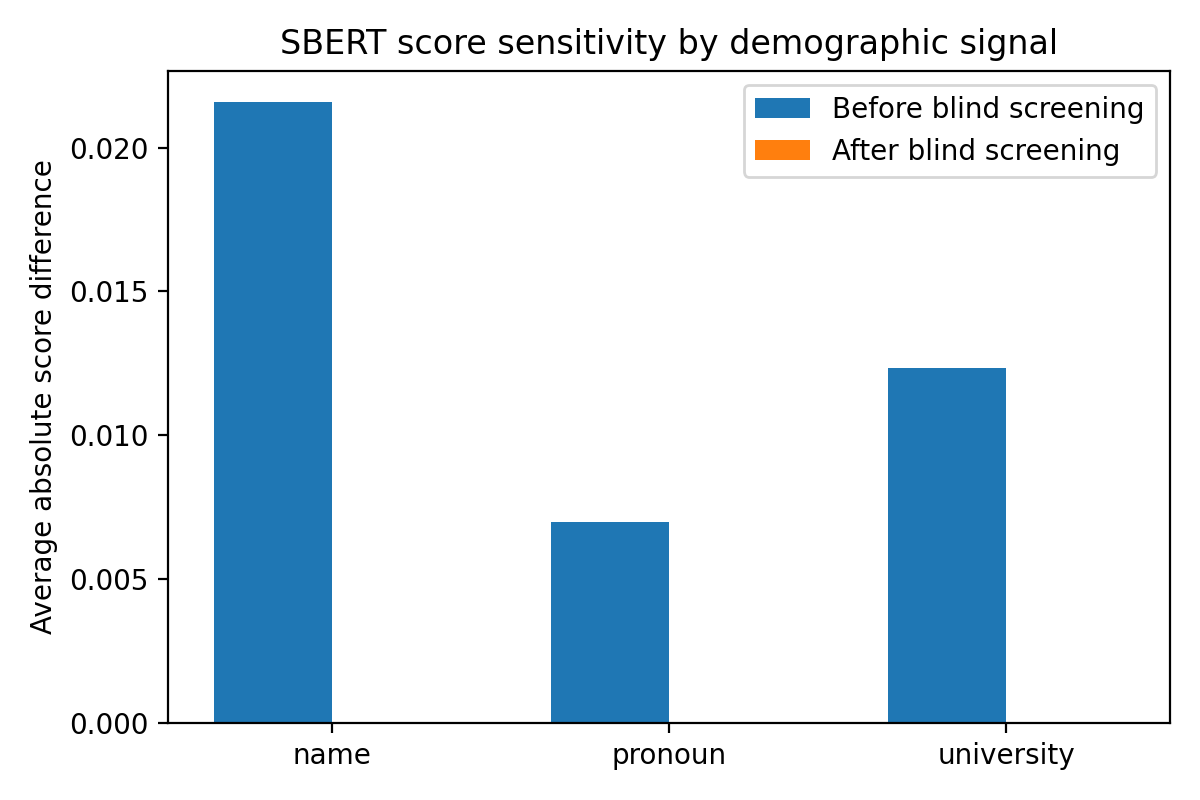
\includegraphics[width=0.95\columnwidth]{figures/fig_before_after_blind.png}
\caption{Average absolute score difference per signal, before and after blind screening. The drop to zero for name and university is partly an artifact of our construction (see Section~\ref{sec:discussion}).}
\label{fig:before_after}
\end{figure}

\subsection{Per-Domain Breakdown}

Figure~\ref{fig:by_domain} shows the average absolute difference broken down by the five domains. The picture is not even: name changes have a bigger effect on the Software Engineering and Finance jobs than on Healthcare, for example. With only one job per domain we cannot read too much into this, but the variation is worth flagging.

\begin{figure}[t]
\centering
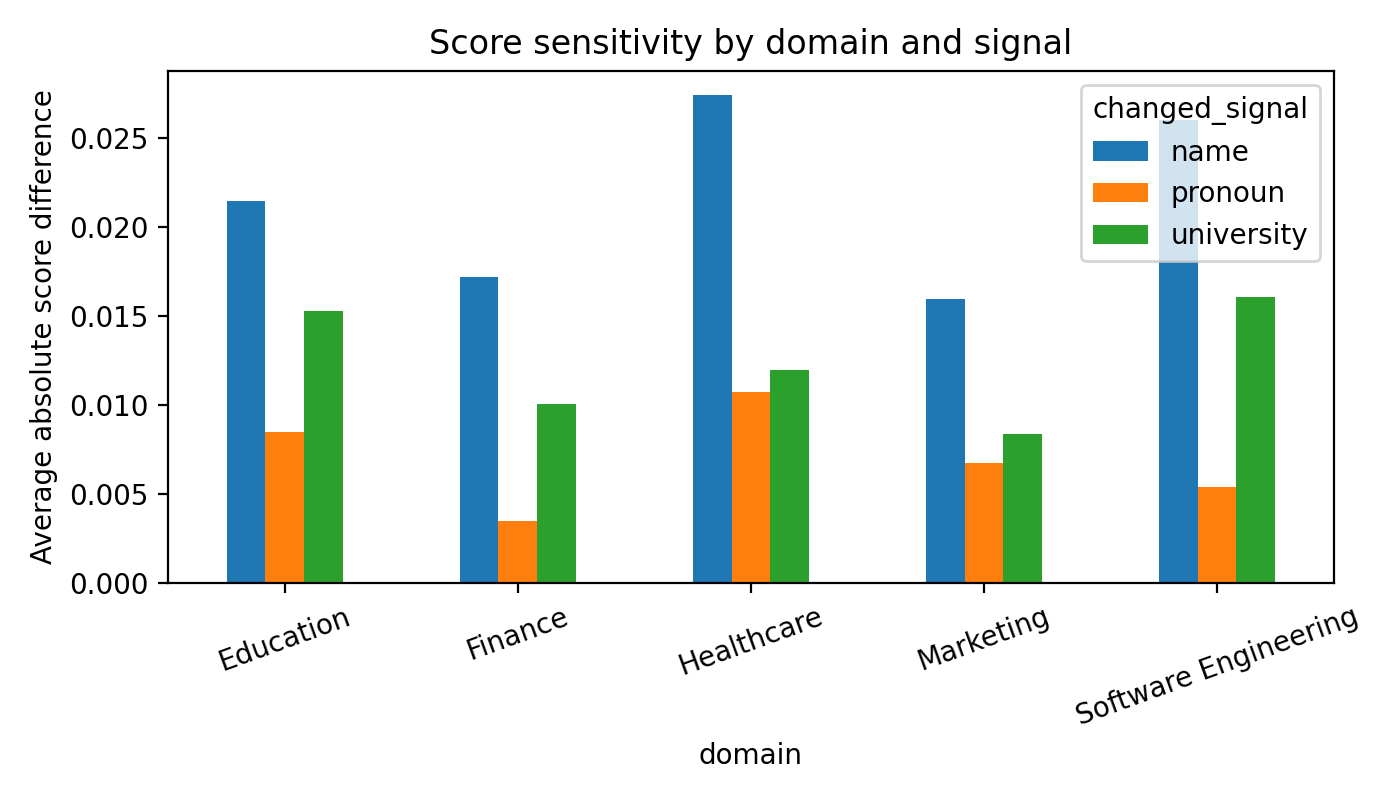
\includegraphics[width=0.95\columnwidth]{figures/fig_by_domain.png}
\caption{Average absolute score difference by domain and signal.}
\label{fig:by_domain}
\end{figure}

\subsection{Compound Signal}

When the name, the pronouns, and the university all change at the same time, the average absolute SBERT score difference is 0.0257. The sum of the three single-signal absolute differences (0.0216 + 0.0070 + 0.0123) is 0.0409. The compound number is smaller than the sum, which suggests that the signals partly cancel each other when combined rather than reinforcing. We do not have enough data to say whether this is a general property or a quirk of the specific counterfactual choices we made.

\subsection{LLM Results}

The LLM result is the most honest negative finding of the project. After switching to sampling and shuffling the prompt option order, FLAN-T5-base stopped defaulting to ``Weak match'' and instead defaulted to ``Strong match'' on all 40 resume-job pairs. The flip rate per demographic signal was 0\% for every signal: not because the model is unbiased, but because it returns the same label no matter what the input is. The label distribution is saturated.

This tells us that FLAN-T5-base at this prompt length is not a useful auditor for resume-job matching. It is responsive to the prompt's listed options (which is why the default label changed when we shuffled them) but not to the actual content of the resume. A larger or instruction-tuned-for-classification model is likely needed to do this audit properly. We list this as future work.

\section{Discussion}
\label{sec:discussion}

The SBERT counterfactual differences are small in absolute terms but are not zero. The bootstrap confidence intervals are clearly above zero, so the model is reacting to the demographic-only change in a measurable way. The most reliable finding by Wilcoxon is for pronouns: small in size, but consistent in direction. Name and university changes are larger on average but the signed shifts go both ways, which we read as ``the model is sensitive to the change, but the direction depends on the specific resume.''

The TF-IDF baseline pushed us to revise an early hypothesis. We expected TF-IDF to show roughly the same pattern as SBERT, which would mean the effect is mostly in the resume text. Instead, TF-IDF shows much smaller shifts and a zero shift for pronouns. So the SBERT sensitivity is mostly being added by the neural embedding, not by word overlap. That is a useful constraint on where the bias lives.

The blind-screening result is the part we want to be most honest about. The 0.000 numbers are forced by the construction of the dataset: when the only difference between two resumes is one word and you delete that word, the embeddings are identical. We treat this as a sanity check rather than a real mitigation result. To test mitigation properly we would need resumes where demographic cues are entangled with the rest of the text.

The LLM section had a similar lesson. Our first run with beam search produced identical outputs because the model returned the first listed option every time. We switched to sampling and shuffled the option order. The model stopped defaulting to ``Weak match'' but immediately started defaulting to ``Strong match'' instead. The flip rate on counterfactuals was zero. The honest reading is that FLAN-T5-base does not pay enough attention to the resume content at this prompt length to be a useful auditor. This is itself a finding: small instruction-tuned LLMs need careful prompt and decoding setup before they can be used in a bias audit, and even then they may not respond to fine-grained text changes.

\section{Limitations}

The dataset is small: 10 base resumes, 5 jobs, 5 domains. Numbers should be read as an audit-style observation, not a claim about real ATS behavior. The counterfactual edits are also stylized; real demographic cues come through writing style, school prestige, addresses, hobbies, and many other paths that we do not edit.

The blind-screening result has the construction problem already discussed. The LLM run uses a small open-source model with a short prompt and is more useful as a probe than as a final answer.

\section{Scope Changes Relative to the Proposal}
\label{sec:scope}

We want to be clear about what changed between the proposal and what we delivered. The proposal promised three mitigation strategies (blind screening, data augmentation, and adversarial debiasing) and an accuracy-vs-fairness comparison. We ended up running blind screening only, and we did not measure an accuracy metric on a held-out task. We added the TF-IDF baseline and the compound-signal audit in response to those gaps. We also added the FLAN-T5-base comparison after the proposal feedback asked us to try a current LLM. Data augmentation and adversarial debiasing are listed as future work in Section~\ref{sec:future}.

\section{Ethical Considerations}

A model that gives different scores to equally qualified applicants because of demographic cues can change who gets an interview. That is the basic ethical concern in this project. We want to flag a few specific points.

First, names, pronouns, and university are only proxies for the demographic and social signals that matter. Real identity is more complex than swapping one field. So even a model that passes our audit could still produce unfair outcomes through other paths.

Second, hiring AI is increasingly regulated. The U.S. Equal Employment Opportunity Commission uses the four-fifths rule as a rough disparate-impact test. New York City Local Law 144 (in effect since 2023) requires bias audits of automated employment decision tools. The EU AI Act classifies hiring AI as high-risk. Our project is not a legal-compliance audit, but it is the kind of counterfactual check that those audits often include.

Third, blind screening can reduce some surface sensitivity but it removes information that some employers find relevant (like the school name). That tradeoff between fairness and information should be made openly, not hidden inside a model.

Finally, Sentence-BERT was trained on web data that carries the same biases as the rest of the internet. Removing fields from the resume does not change anything inside the embedding model. So even with blind screening at the input, the underlying model can still be biased.

\section{Reproducibility}

The code, data, and result files are in a public GitHub repository:\\
\url{https://github.com/skandul2-dot/bias-aware-resume-matching-final}

The \texttt{data/} folder has the base resumes, the counterfactual variants, and the job descriptions. The \texttt{notebooks/} folder has seven Colab notebooks, one per pipeline step. The \texttt{results/} folder has the CSV outputs (SBERT scores, fairness comparison, blind-screening results, TF-IDF baseline, compound-signal comparison, statistical tests, LLM decisions, and LLM flip summary). The \texttt{report/} folder has this report.

The exact model versions are \texttt{sentence-transformers/all-MiniLM-L6-v2} and \texttt{google/flan-t5-base}. We set \texttt{random.seed(42)} and \texttt{torch.manual\_seed(42)} in the LLM notebook.

\section{Future Work}
\label{sec:future}

The two pieces from the original proposal that we did not deliver are the obvious next steps:

\textbf{Data augmentation.} Train (or fine-tune) on a dataset that includes counterfactual pairs as positive examples of equivalence, so the model learns that swapping a name should not change the score.

\textbf{Adversarial debiasing.} Add an adversary network that tries to predict the demographic signal from the embedding, and train the main model to fool it.

Beyond those, the experiment would be more convincing on a larger dataset with multiple jobs per domain, more counterfactual names per resume, and an external accuracy metric (a held-out set of human-judged matches) so we could measure the fairness-accuracy tradeoff that the proposal asked about.

\section{Conclusion}

We built a small bias-aware resume-job matching pipeline using Sentence-BERT, ran a counterfactual audit on demographic-only changes, added a TF-IDF baseline, a compound-signal audit, statistical tests, and a comparison with FLAN-T5-base. SBERT scores react to all three demographic changes, with the pronoun shift being the most directionally consistent. TF-IDF reacts much less, which suggests the SBERT sensitivity comes from the embedding rather than from word overlap. The compound change moves the score less than the sum of single-signal changes, so the signals partly cancel. Blind screening drops everything to zero, which on this dataset is a construction artifact and not a real mitigation result. FLAN-T5-base saturates on a single label and is not a useful auditor at this size. Even with a small, controlled dataset the audit picks up clear demographic sensitivity that the model should not have.

\bibliography{references}
\bibliographystyle{icml2022}

\begin{thebibliography}{9}

\bibitem[Bertrand and Mullainathan(2004)]{bertrand2004emily}
Bertrand, M.\ and Mullainathan, S.
\newblock Are Emily and Greg more employable than Lakisha and Jamal? A field experiment on labor market discrimination.
\newblock {\em American Economic Review}, 94(4):991--1013, 2004.

\bibitem[Bolukbasi et al.(2016)]{bolukbasi2016man}
Bolukbasi, T., Chang, K.-W., Zou, J., Saligrama, V., and Kalai, A.
\newblock Man is to computer programmer as woman is to homemaker? Debiasing word embeddings.
\newblock In {\em NeurIPS}, 2016.

\bibitem[Caliskan et al.(2017)]{caliskan2017semantics}
Caliskan, A., Bryson, J. J., and Narayanan, A.
\newblock Semantics derived automatically from language corpora contain human-like biases.
\newblock {\em Science}, 356(6334):183--186, 2017.

\bibitem[Chung et al.(2022)]{chung2022scaling}
Chung, H.~W., Hou, L., Longpre, S., et al.
\newblock Scaling instruction-finetuned language models.
\newblock {\em arXiv preprint arXiv:2210.11416}, 2022.

\bibitem[De-Arteaga et al.(2019)]{dearteaga2019bias}
De-Arteaga, M., Romanov, A., Wallach, H., Chayes, J., Borgs, C., Chouldechova, A., et al.
\newblock Bias in bios: A case study of semantic representation bias in a high-stakes setting.
\newblock In {\em FAT*}, 2019.

\bibitem[Kusner et al.(2017)]{kusner2017counterfactual}
Kusner, M.~J., Loftus, J., Russell, C., and Silva, R.
\newblock Counterfactual fairness.
\newblock In {\em NeurIPS}, 2017.

\bibitem[Qin et al.(2018)]{qin2018enhancing}
Qin, C., Zhu, H., Xu, T., Zhu, C., Jiang, L., Chen, E., and Xiong, H.
\newblock Enhancing person-job fit for talent recruitment: An ability-aware neural network approach.
\newblock In {\em SIGIR}, pp.\ 25--34, 2018.

\bibitem[Reimers and Gurevych(2019)]{reimers2019sentence}
Reimers, N.\ and Gurevych, I.
\newblock Sentence-BERT: Sentence embeddings using siamese BERT-networks.
\newblock In {\em EMNLP}, pp.\ 3982--3992, 2019.

\bibitem[Wilson and Caliskan(2024)]{wilson2024gender}
Wilson, K.\ and Caliskan, A.
\newblock Gender, race, and intersectional bias in resume screening via language model retrieval.
\newblock In {\em AAAI/ACM AIES}, volume~7, pp.\ 1578--1590, 2024.

\end{thebibliography}

\end{document}
